\section{Results}

This section shows the results of the environment model and the i2a implementation. Also it shows the performance of i2a over the model-free baseline and the copy model.

%In the following the performance of I2A over the model-free baseline and the copy model is shown. Also the predicted rollouts of the environment model.

\subsection{Environment Model Training}

Our trained environment model is an imperfect model, which is in most cases able to predict a few steps into the future, but it is bad at predicting far into the future.\\





\begin{figure}[H] 
  \centering   
  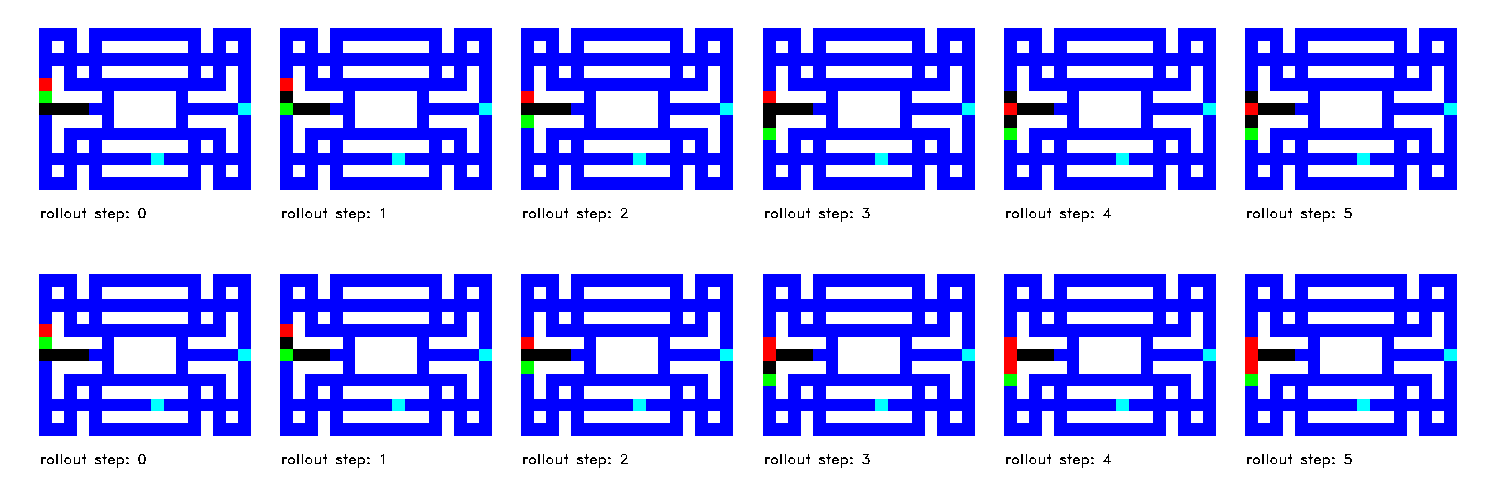
\includegraphics[width=\columnwidth]{./Images/env_model_rollouts.png}
  \caption{Environment model rollouts, top true observations, bottom predicted observations, rollout steps from left to right} 
  \label{fig:environment_model_rollouts} 
\end{figure} 



Figure \ref{fig:environment_model_rollouts} shows the true next observations in the upper row and the predicted next observations in the lower row. From left to right it shows the rollout steps, the prediction is always based on the previous rollout step. In the beginning the prediction is quite good but the errors accumulate, leading to prediction errors like the one in rollout step 3 of figure \ref{fig:environment_model_rollouts}. The environment model is unsure where the ghost, the red points, are moving and as a result it predicts the ghost at two positions.\\



TODO check numbers\\
The environment model was trained for 2000 million frames, on a Titan Xp GPU for ~160 hours with around 3470 frames per second. As optimizer we used Adam with a learning rate of $10^{-4}$ and a weight decay of 0.01. The batch size was 500 and we weighted the reward loss with a coefficient of 0.01 compared to the frame loss. To train the environment model with a representative set of observations, we used as described in section \ref{sec:env_model} a pretrained a2c policy to create samples of pairs of observation and reward.
%1352.8min + 8274.3
% main_train_environment_model.py --env-name HuntMiniPacmanNoFrameskip-v0 --environment-model MiniModel --lr 1e-4 --save-interval 100 --batch-size 500 --sample-memory-size 1500 --num-episodes 300000000 --port 5028

\begin{figure}[H] 
  \centering   
  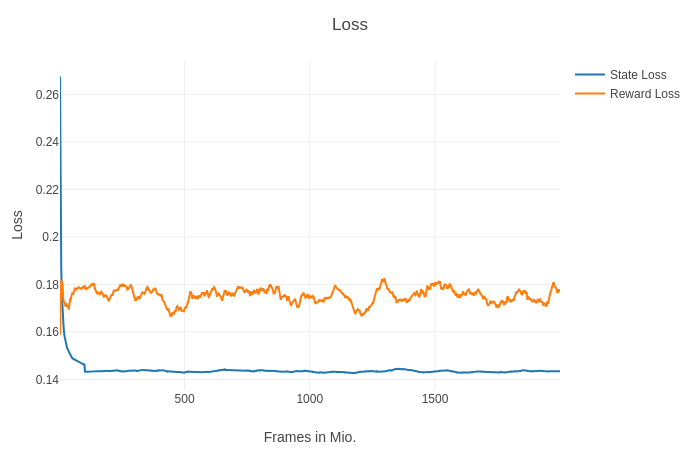
\includegraphics[width=0.7\columnwidth]{./Images/hunt_env_loss_curve.png}
  \caption{Environment model loss curve} 
  \label{fig:env_model_loss} 
\end{figure} 

The figure \ref{fig:env_model_loss} shows the loss curve of the environment model training. It seems as if the loss stagnates very soon, but the main advantage in correct predictions is learned in the part with small loss changes. To learn the general structure of the maze is easy but to predict the correct position of the player and the ghosts is really hard, but has only a small impact on the loss.\\




\subsection{I2A MiniPacman Results}

In this section we demonstrate the performance of our reinforcement learning agent and compare our results with the results of the "imagination augmented agent for deep reinforcement learning" paper \cite{I2A}.
%In this section we compare the performance of our reinforcement learning agent to the results of the paper.
To do so we trained three different agents, an a2c model-free baseline, the copy model and the i2a agent on the reinforcement learning task MiniPacman in the modes "Regular" and "Hunt".\\
%To do so we trained MiniPacman in the mode 'Regular' and 'Hunt' with 3 different agents, a A2C model-free baseline, the copy model and the I2A agent.
%To compare the performance, we trained MiniPacman Hunt with a A2C model-free baseline, the copy model and I2A agent.\\

As baseline for our implementation we used the a2c reinforcement learning pytorch implementation of Ilya Kostrikov\cite{pytorchrl}.

%\begin{comment}
\begin{figure}[H] 
    \centering
    \begin{subfigure}[b]{0.45\textwidth}
        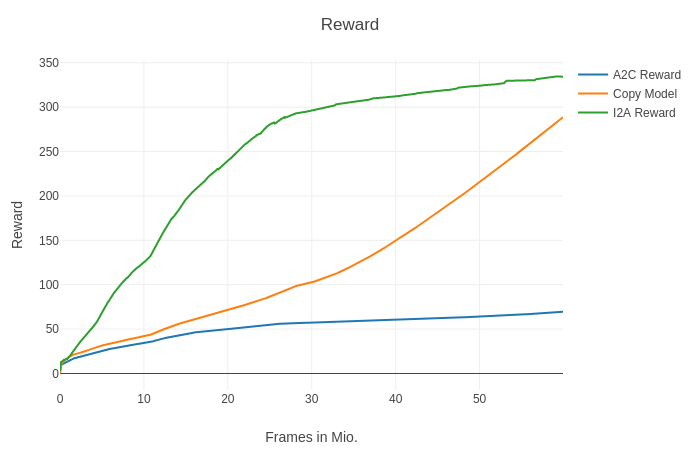
\includegraphics[width=\textwidth]{./Images/regular_rewards_compare.png}
  		\caption{Received reward of i2a run with 2 rollouts (green), model-free a2c baseline (blue) and copy model (orange).} 
  		\label{fig:mini_pacman_regular_rewards} 
    \end{subfigure}
	~ %add desired spacing between images, e. g. ~, \quad, \qquad, \hfill etc.       
    \begin{subfigure}[b]{0.45\textwidth}
        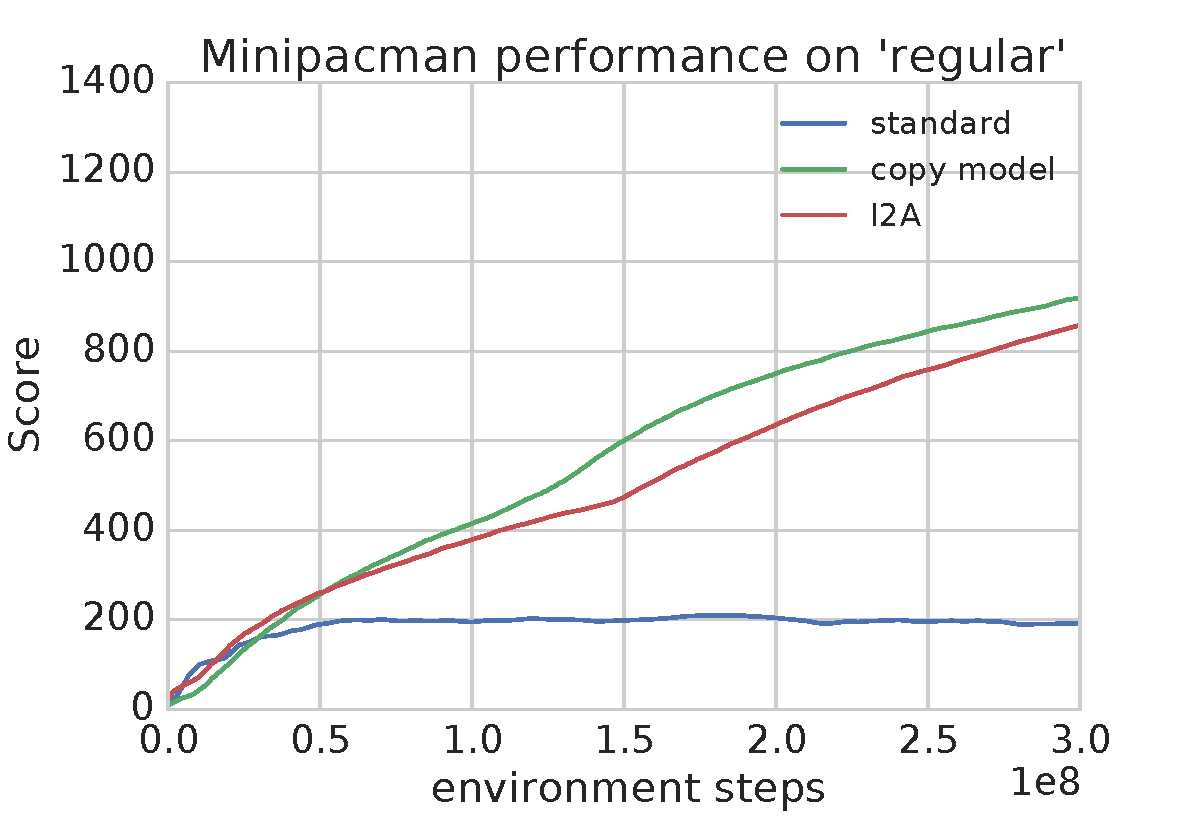
\includegraphics[width=\textwidth]{./Images/minipacman_regular.pdf}
  		\caption{Received rewards from the "imagination augmented agent for deep reinforcement learning" paper \cite{I2A}.} 
  		\label{fig:mini_pacman_regular_original_rewards}
    \end{subfigure}
    
    \caption{Learning curves for different agents on the task MiniPacman Regular}\label{fig:mini_pacman_regular}
\end{figure}

%\end{comment}

Figure \ref{fig:mini_pacman_regular_rewards} shows our training results for the reinforcement learning task MiniPacman Regular. The a2c baseline is clearly outperformed by the copy model and the i2a model, but there is no performance improvement of the i2a over the copy model. The performance improvement therefore only corresponds to the parameter increasement and not to the imagined rollouts. 
Our results match with the results of the original i2a paper which also have no improvement of i2a over the copy model in the mode "Regular" as shown in figure \ref{fig:mini_pacman_regular_original_rewards}.
We trained our agents for 100 million frames on a Titan Xp which took for the a2c baseline $\sim$16 hours, for the copy model $\sim$36 hours and for the i2a $\sim$63 hours.


\begin{figure}[H] 
    \centering
    \begin{subfigure}[b]{0.45\textwidth}
        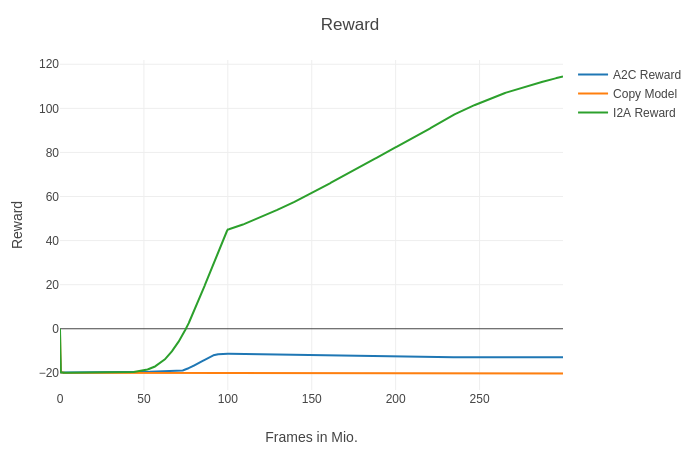
\includegraphics[width=\textwidth]{./Images/hunt_rewards_compare.png}
  		\caption{Received reward of I2A run with 2 rollouts (green), model-free A2C baseline (blue) and copy model (orange).} 
  		\label{fig:mini_pacman_hunt_rewards} 
    \end{subfigure}
	~ %add desired spacing between images, e. g. ~, \quad, \qquad, \hfill etc.       
    \begin{subfigure}[b]{0.45\textwidth}
         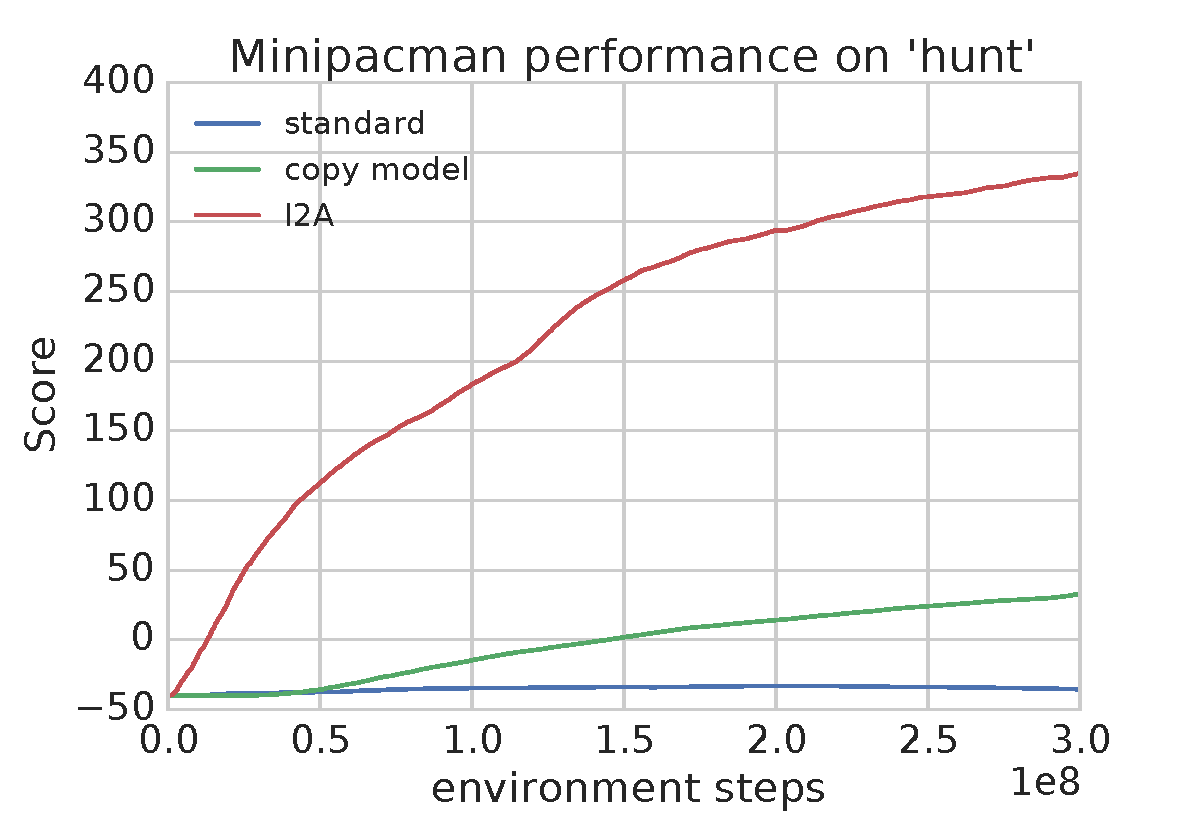
\includegraphics[width=\textwidth]{./Images/minipacman_ghosthunt.pdf}
		 \caption{Received rewards from the "imagination augmented agent for deep reinforcement learning" paper \cite{I2A}.} 
		\label{fig:mini_pacman_hunt_original_rewards} 
    \end{subfigure}
    
    \caption{Learning curves for different agents on the task MiniPacman Hunt}\label{fig:mini_pacman_hunt}
\end{figure}

The results of the trained agents on MiniPacman in Hunt mode are shown in figure \ref{fig:mini_pacman_hunt}. As you can see i2a outperforms clearly the a2c baseline and the copy model shown in figure \ref{fig:mini_pacman_hunt_rewards}.
As before our results match the ones from the paper, see figure \ref{fig:mini_pacman_hunt_original_rewards}, only the maximum reward we reached with our i2a agent is not as high as the results of the original paper.
This difference could be caused by the fact that they use a rollout length of 5 and we only a rollout length of 2.
We trained MiniPacman Hunt for 300 million frames on a Titan Xp  which took for the a2c baseline $\sim$48 hours, for the copy model $\sim$94 hours and for the i2a $\sim$215 hours.\\ 
%A possible reason for this difference is that they use in the paper a rollout lenght of 5 and we use only a rollout length of 2.


The reproduced results from the paper support the statement that the performance gap between i2a and baselines is high for tasks where the rewards are sparse and where planning ahead is important to avoid irreversible actions, as for example move pacman to a position where he gets enclosed by ghosts.
%Hunt due to it's sparse reward and the increasing number of ghosts is a more planning related problem as MiniPacman in Regular mode.



%main.py --algo i2a --env HuntMiniPacmanNoFrameskip-v0 --num-processes 128 --port 5555 --log-dir /tmp/gym/Hunt_AfterBugfix --num-steps 10 --entropy-coef 0.02 --distill-coef 0.3 --num-stack 1 --use-class-labels
%TODO compare result with the one of the i2a paper.



\begin{comment}
\begin{figure}[H] 
  \centering   
  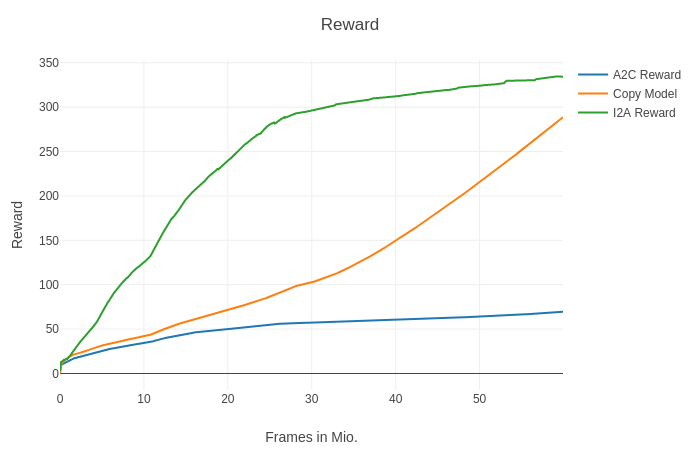
\includegraphics[width=0.7\columnwidth]{./Images/regular_rewards_compare.png}
  \caption{Reached rewards on the environment MiniPacman Hunt. Green curve I2A run with 2 rollouts, blue curve model-free A2C baseline and orange curve copy model results.} 
  \label{fig:mini_pacman_regular_rewards} 
\end{figure} 


\begin{figure}[H] 
  \centering   
  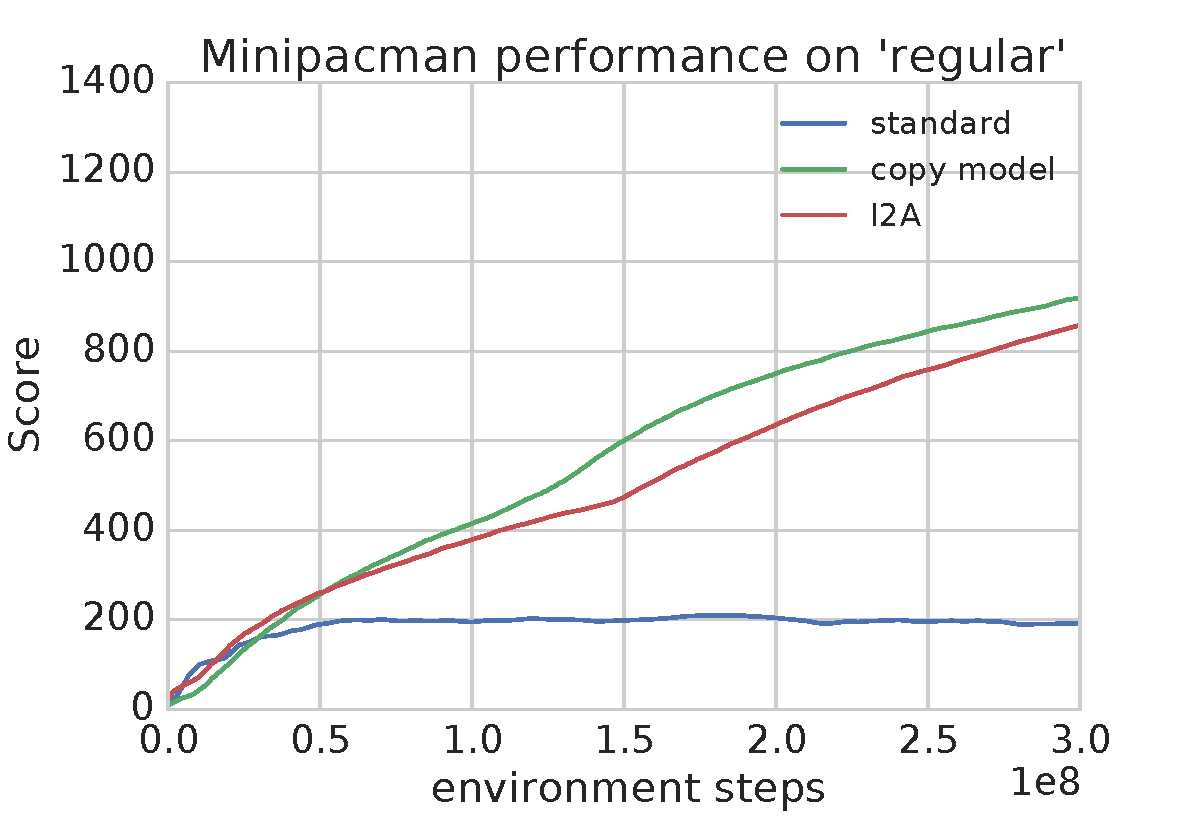
\includegraphics[width=0.7\columnwidth]{./Images/minipacman_regular.pdf}
  \caption{Results from the paper} 
  \label{fig:mini_pacman_regular_original_rewards} 
\end{figure} 
\end{comment}

\begin{comment}
\begin{figure}[H] 
  \centering   
  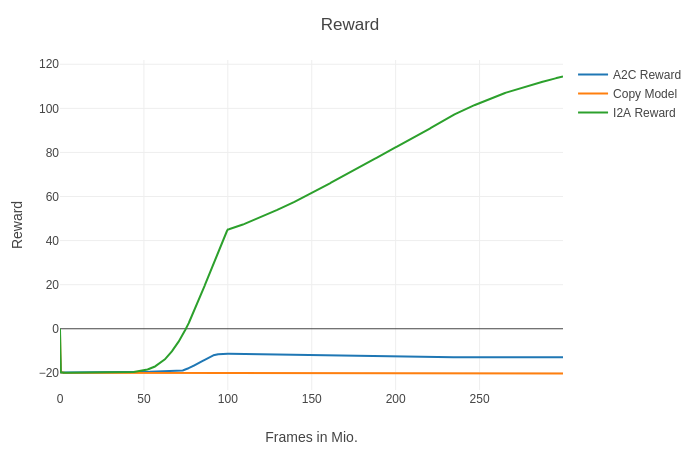
\includegraphics[width=0.9\columnwidth]{./Images/hunt_rewards_compare.png}
  \caption{Reached rewards on the environment MiniPacman Hunt. Green curve I2A run with 2 rollouts, blue curve model-free A2C baseline and orange curve copy model results.} 
  \label{fig:mini_pacman_hunt_rewards} 
\end{figure} 

\begin{figure}[H] 
  \centering   
  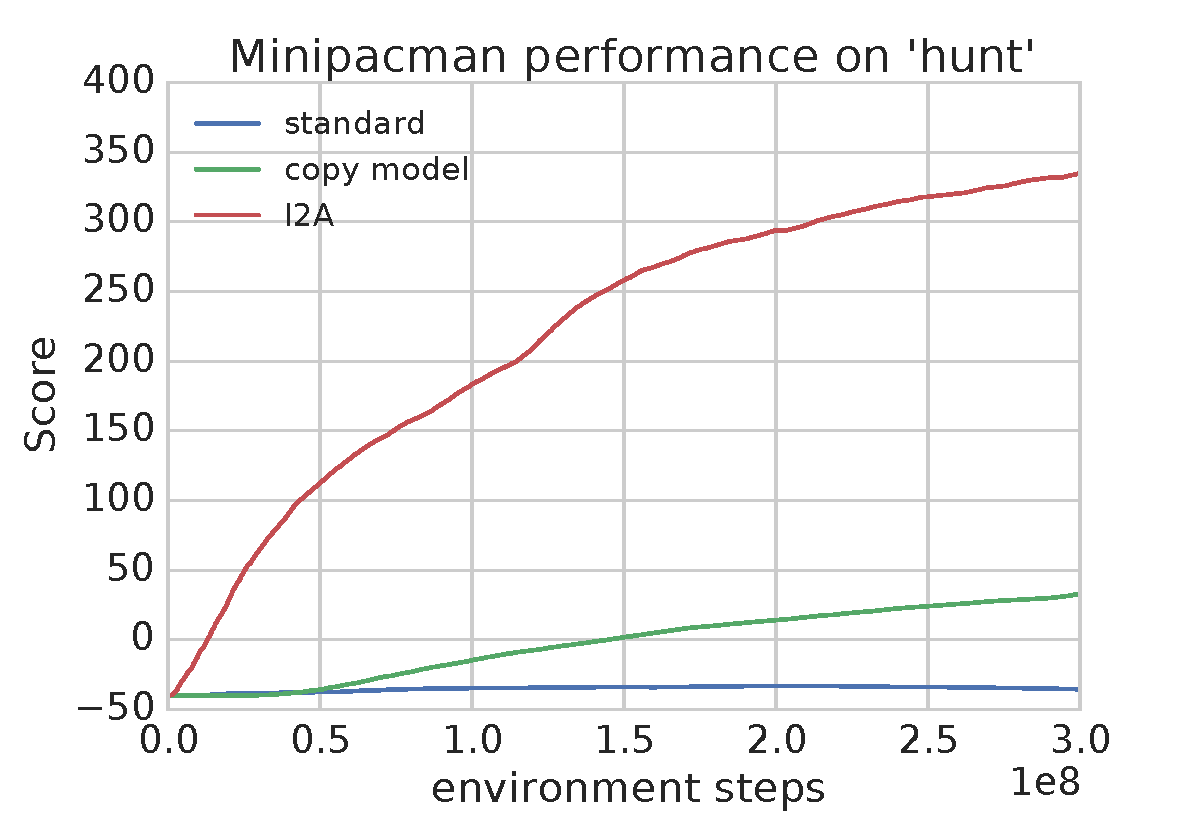
\includegraphics[width=0.9\columnwidth]{./Images/minipacman_ghosthunt.pdf}
  \caption{Reached rewards on the environment MiniPacman Hunt. Green curve I2A run with 2 rollouts, blue curve model-free A2C baseline and orange curve copy model results.} 
  \label{fig:mini_pacman_hunt_original_rewards} 
\end{figure} 
\end{comment}